\chapter{Metodologia}

A pergunta de pesquisa deste estudo investiga a dinâmica de processos epidemiológicos em redes de mobilidade temporais, em comparação com redes de mobilidade estáticas, com ênfase na variação da resolução temporal, ou seja, na granularidade da rede \cite{Pedrycz2002}. A metodologia envolve a variação da resolução temporal, desde uma rede por dia (melhor resolução - \textit{baseline}) até resoluções piores, como uma rede a cada 2 ou 3 dias. Observaremos o modelo \textit{SIR Euleriano} para compreender o impacto das diferentes escalas de tempo na propagação da doença. Posteriormente, compararemos os resultados obtidos em diferentes resoluções com o resultado da melhor resolução, utilizando alguma norma. Essa comparação é fundamental para avaliar a acurácia das modelagens em diferentes escalas de tempo e, assim, aprimorar as estratégias de controle epidemiológico.

\section{Metapopulações}

As metapopulações são um conceito fundamental em ecologia que descrevem grupos de populações de uma mesma espécie ocupando diferentes áreas geograficamente separadas e interagindo em algum nível. Esse termo foi cunhado por \citeonline{levins1969demographic} quando desenvolveu um modelo para entender a dinâmica populacional de pragas de insetos em campos agrícolas. No entanto, esse conceito tem sido amplamente aplicado em ecologia para compreender como as espécies respondem a ambientes fragmentados, sejam eles fragmentados naturalmente, como ocorre em ilhas, ou como resultado de ações humanas, como a destruição de habitats naturais.

Uma metapopulação consiste em várias populações distintas que ocupam áreas de habitat adequadas, incluindo algumas áreas ocasionalmente desocupadas. Cada população interage relativamente de forma independente com as outras e está sujeita a eventos demográficos aleatórios que podem levar à extinção local. À medida que as populações diminuem, aumenta o risco de desaparecimento devido a fatores diversos. No entanto, a metapopulação como um todo é mais estável, pois indivíduos de populações bem-sucedidas frequentemente migram para áreas desocupadas devido à extinção de outras populações, um processo chamado \textit{efeito de resgate}, crucial para a manutenção da metapopulação como um todo.

\begin{figure}[!h]
    \centering
    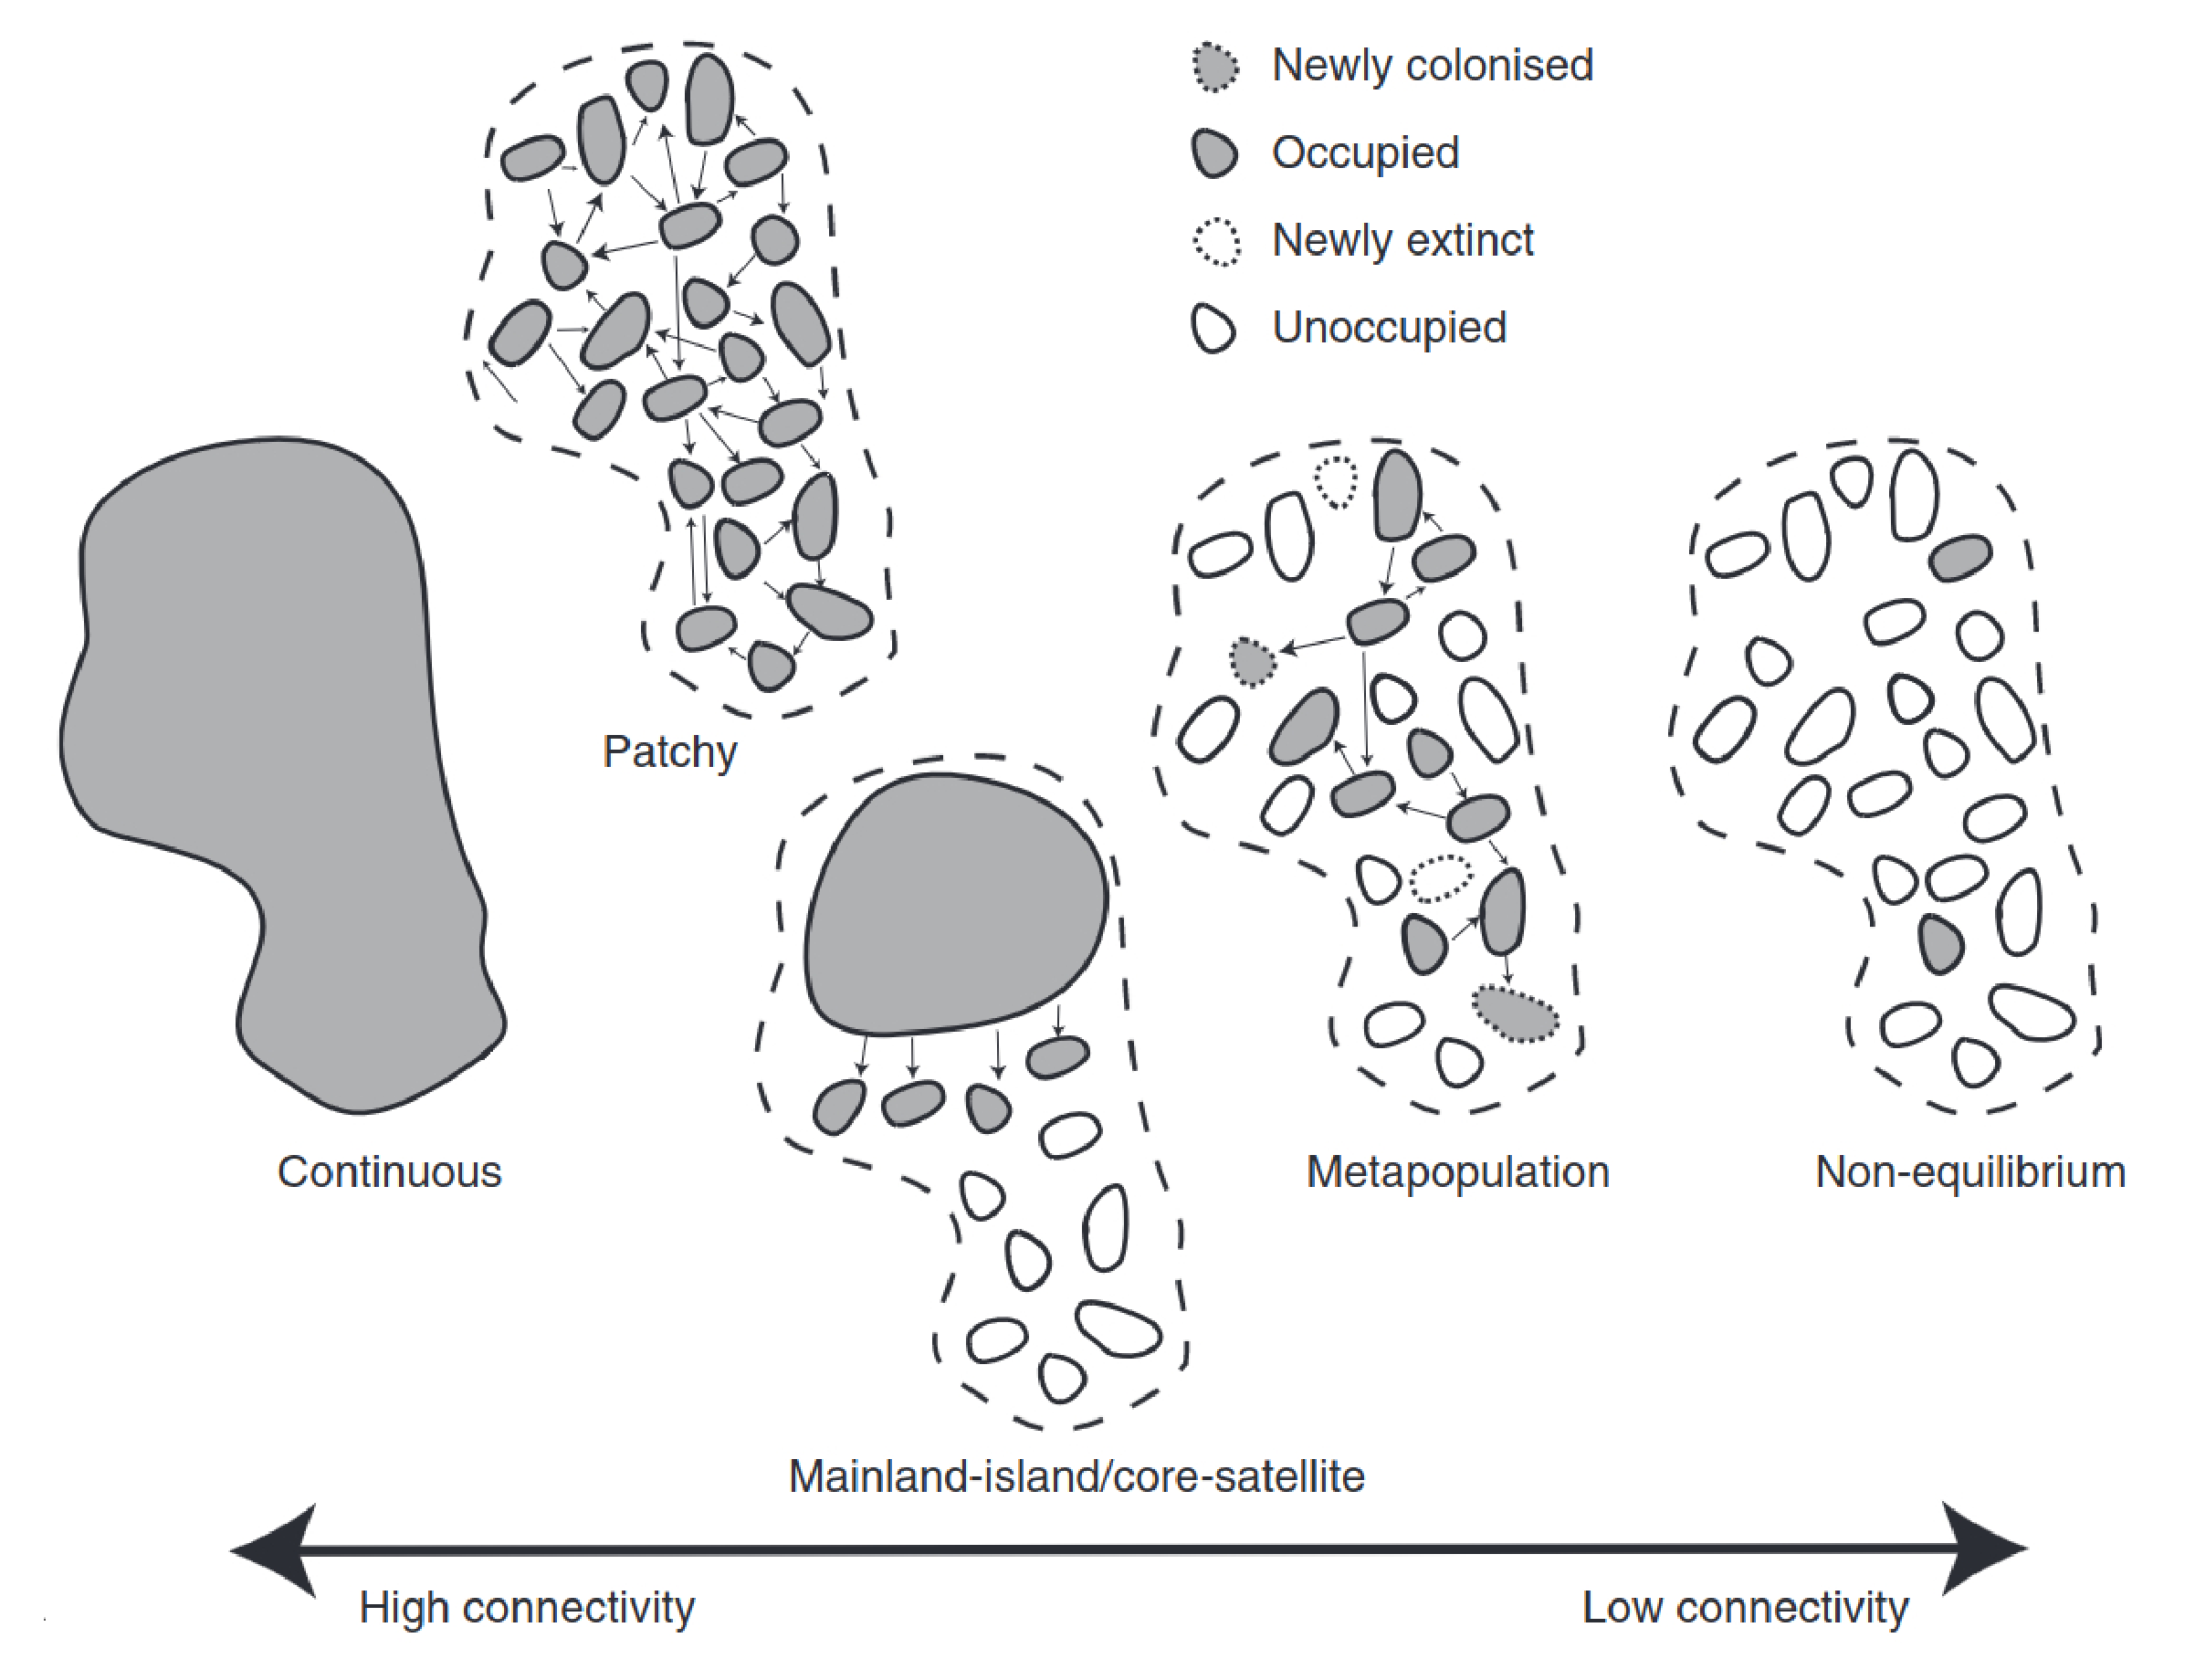
\includegraphics[width=10.8cm]{figures/metapop.pdf}
    \caption{Quatro tipos de modelos de metapopulação \cite{Harrison2008} com diferentes níveis de conectividade, adaptado de \citeonline{Nouhuys2009}.}
    \label{fig:metapopulations}
\end{figure}

\newpage

O termo \textit{subpopulações} é frequentemente usado de forma sinônima com \textit{populações locais} em contextos de metapopulação \cite{HanskiGaggiotti2004}. Estas subpopulações ou populações locais são grupos de indivíduos de uma espécie que ocupam áreas específicas dentro da metapopulação maior e estão interligados por meio de movimento entre essas áreas. Elas desempenham um papel fundamental na dinâmica da metapopulação, influenciando a sobrevivência e a distribuição da espécie em todo o conjunto de áreas ocupadas.

A fusão de redes e modelos epidemiológicos aos modelos de metapopulação oferece uma perspectiva mais abrangente para a compreensão da propagação de doenças infecciosas em sistemas complexos. As metapopulações podem ser pensadas como nós de uma rede complexa de manchas (\textit{patchies} em inglês) espaciais, onde os links codificam os fluxos humanos de um lugar para outro e são responsáveis pela transmissão entre manchas \cite{HAGENAARS2004349}, reforçando a importância da abordagem integrada. Esses modelos de metapopulação fornecem a estrutura básica para analisar a interação entre hospedeiros em diferentes áreas, presumindo uma mistura homogênea e contatos aleatórios localmente, o que permite uma visão geral das populações ao longo do tempo, calibrada com dados censitários.

No contexto de nosso projeto, incorporamos esses conceitos para entender a dinâmica de transmissão de doenças infecciosas em uma escala mais ampla. Ao combinar modelos de metapopulação com modelos epidemiológicos, podemos examinar como a transmissão de doenças ocorre localmente, levando em consideração a mobilidade das espécies hospedeiras. Essa abordagem é fundamental para entender os mecanismos de propagação de doenças infecciosas em nosso sistema e desenvolver estratégias eficazes de prevenção e controle, especialmente em sistemas complexos onde a conectividade entre populações desempenha um papel crucial.

\begin{figure}[!h]
    \centering
    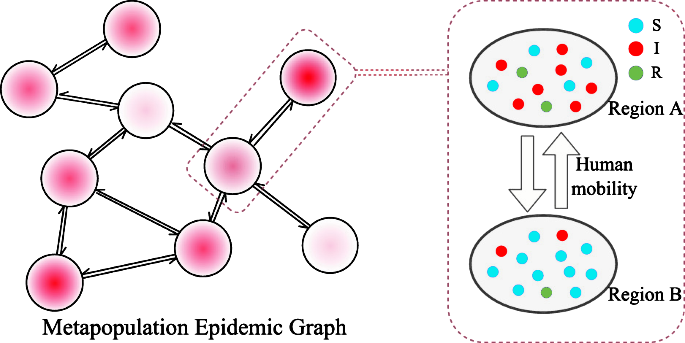
\includegraphics[width=10.8cm]{figures/metapopSIR.png}
    \caption{Modelo SIR em uma rede metapopulacional de manchas, adaptado de \citeonline{Cao2023}.}
    \label{fig:metapopulations}
\end{figure}

\newpage

\section{Modelos de movimento de hospedeiro}

Modelos de movimentação de hospedeiros, como os Eulerianos e Lagrangianos, são essenciais para simular a movimentação dentro de redes metapopulacionais. Enquanto os Eulerianos não rastreiam o comportamento individual e são adequados para descrever a migração animal, os Lagrangianos seguem os indivíduos e são mais adequados para descrever o comportamento de deslocamento humano \cite{Citron2021}.

Para compreender a difusão geográfica das doenças em escalas espaciais variadas devido à mobilidade humana, a modelagem epidêmica adota a dinâmica de reação-difusão na metapopulação \cite{Dirk2013}. Em nosso estudo, empregamos o modelo Euleriano para descrever a difusão de hospedeiros entre metapopulações \cite{Citron2021}, representado pela equação diferencial a seguir:
{\large
\begin{center}
\begin{equation}
    \frac{dN_{i}}{dt} = -\sum_{j=1}^{K} f_{i, j} N_{i} + \sum_{j=1}^{K} f_{j, i} N_{j},
\end{equation}
\end{center}}

A mobilidade dos agentes entre as manchas é governada por uma matriz ponderada, onde a probabilidade de um agente localizado em $i$ se deslocar para $j$ é diretamente proporcional ao fluxo. Nesse cenário, $N_{i}$ representa o número de hospedeiros em $i$, enquanto $K$ corresponde ao total de subpopulações. A taxa $f_{i, j}$, que descreve as taxas de movimentação entre as subpopulações, é representada por uma matriz adjacência ponderada $KxK$. 

O número total de hospedeiros permanece constante ao longo do tempo:
{\large
\begin{center}
\begin{equation}
    N = \sum_{i=1}^{K} N_{i}.
\end{equation}
\end{center}}

Introduzindo a dinâmica da reação, combinamos o modelo SIR com o Euleriano, gerando um conjunto de equações $3K$ para as subpopulações:

{\large
\begin{equation}
\begin{cases}
    \frac{dS_{i}}{dt} = -\beta_{i} \frac{S_{i}I_{i}}{N_{i}} -\sum_{j=1}^{K} f_{ i, j} S_{i} + \sum_{j=1}^{K} f_{j, i} S_{j}, \\
    \frac{dI_{i}}{dt} = \beta_{i} \frac{S_{i}I_{i}}{N_{i}} - \gamma I_{i} -\sum_{j=1} ^{K} f_{i, j} I_{i} + \sum_{j=1}^{K} f_{j, i} I_{j}, \\
    \frac{dR_{i}}{dt} = \gamma I_{i} -\sum_{j=1}^{K} f_{i, j} R_{i} + \sum_{j=1}^{ K} f_{j, i} R_{j}.
\end{cases}
\end{equation}}

Assim, em cada mancha $i$, a soma de $S_{i}$, $I_{i}$ e $R_{i}$ é igual a $N_{i}$, desempenhando um papel crucial na análise da dinâmica das doenças em uma metapopulação.

\section{Dados de mobilidade}
Os dados de mobilidade, provenientes de diversas fontes, como telefones celulares e itinerários aéreos, registram o movimento das pessoas, fornecendo insights sobre a disseminação de doenças em uma localidade. Em nossa investigação, utilizamos os dados de \citeonline{Baidu}, que monitoram os movimentos entre 340 cidades chinesas de janeiro a fevereiro de 2020 e categorizam a mobilidade como entradas e saídas por província e cidade na China.

Esses dados de mobilidade populacional rastreiam o movimento das pessoas no espaço, permitindo a exploração da tendência espacial de propagação no início da pandemia do COVID-19. O Baidu oferece serviços de localização baseados em GPS, endereços IP, torres de sinalização, Wi-Fi, além de uma variedade de aplicativos e softwares móveis. Eles foram utilizados para analisar a mobilidade da população durante o período do Ano Novo Chinês \cite{HU2020130}.

No contexto da análise, foram consideradas 60 matrizes de entrada e 60 matrizes de saída, cada uma com dimensões originais de $368 \times 369$, correspondendo aos dias de janeiro a fevereiro de 2020. Estas matrizes foram submetidas a um pré-processamento conduzido pela investigação de \citeonline{FreitasSTZM22}, resultando em dimensões de $303 \times 303$.

No entanto, mesmo após o pré-processamento (que serviu para retirar nós com fluxo nulo), ainda existiam lacunas nos fluxos de dados. Posteriormente, aplicamos a normalização das matrizes, com a das matrizes de entrada realizada pelas colunas e a das matrizes de saída pelas linhas, de forma que a soma dos elementos desses eixos totalizasse 100\%.

Para solucionar essa questão, adotamos uma abordagem que envolveu o cálculo dos desvios das taxas de entrada e saída em relação a 100\%. Identificamos os elementos existentes nas matrizes, considerando as colunas para entrada e as linhas para saída. Com base nessas informações, calculamos valores parciais de fluxos para corrigir os desvios e preencher as lacunas nos fluxos existentes, abordando essa correção coluna por coluna ou linha por linha. Esse processo de refinamento contribuiu significativamente para a integridade e estabilidade do nosso modelo SIR Euleriano.